\noindent Linux Installation\textsuperscript{**}: Begin by ensuring that you have Virtual Box installed on your system\cite{LinuxVirtualBoxInstall}, if not type:
\begin{lstlisting}[language=bash]
    $ sudo apt-get install virtualbox
\end{lstlisting}
%\vfill
\let\thefootnote\relax\footnotetext{\textsuperscript{**} \textit{Snap install is not available for all Linux Distros, this is expected to work on Ubuntu and Debian flavours}}
%---------------------
\subsubsection{Create Virtual Machine}
\begin{figure}[!htb]
    \centering
    %\insertcode{Scripts/example.pl}{Nena would be proud.} % The first argument is the script location/filename and the second is a caption for the listing
    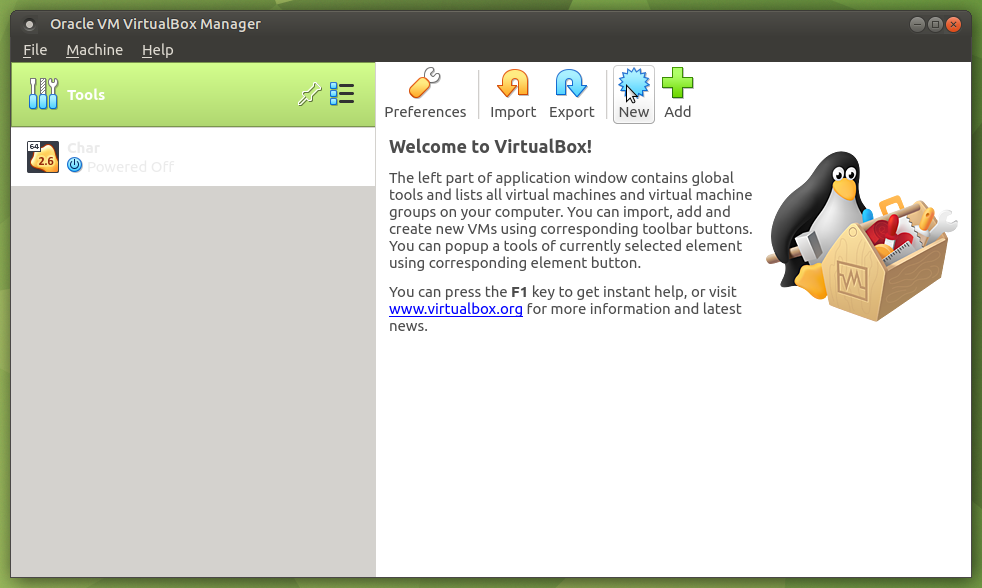
\includegraphics[width=0.752\textwidth]{images/00-0.png}\\[0cm]  
    \caption[Virtual Box]{New Virtual Machine Setup}
    %from \url{http://localhost:3000/}).} % The text in the square bracket is the caption for the list of figures while the text in the curly brackets is the figure caption
    \label{fig:00-01 - Linux Virtual Box New VM} 
\end{figure}
Begin by Creating a new Virtual Machine. To do this click on the blue icon
labelled new as shown in Figure \vref{fig:00-01 - Linux Virtual Box New VM}.

%---------------------
\subsubsection{Name \& Operating System}
\begin{figure}[!htb]
    \centering
    %\insertcode{Scripts/example.pl}{Nena would be proud.} % The first argument is the script location/filename and the second is a caption for the listing
    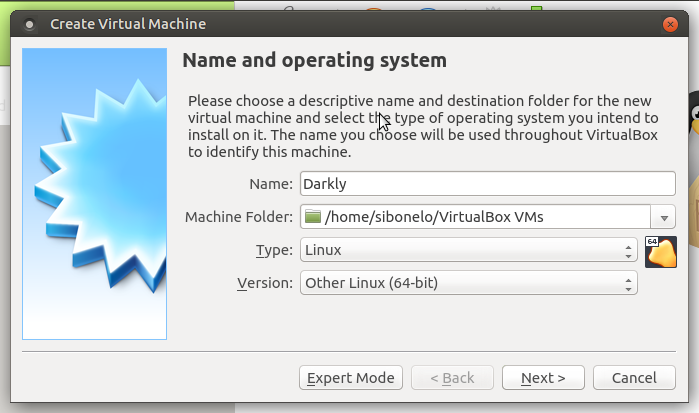
\includegraphics[width=0.752\textwidth]{images/00-01.png}\\[0cm]  
    \caption[Virtual Box]{Setup Of Operating System Type and Name}
    \label{fig:00-02 - Linux Virtual Box Operating System} 
\end{figure}
You have to give your Virtual Machine a new name, I have chosen 'Darkly'. Make
sure to pick a folder for storage of the Virtual Machine or leave it to the
default provided by Virtual Box.

You will have to choose the 'type' of machine you are creating. At this point
you must select 'Linux' as this is what the Darkly.iso is based from. You will
be given options or 'flavours' to choose from. Pick 'Other 64-bit'. This is
best shown in Figure ~\Vref{fig:00-02 - Linux Virtual Box Operating System}.

Please do take note that the Darkly VM will not work if it is not 64-bit.

%---------------------
\subsubsection{Memory Size}
\begin{figure}[!htb]
    \centering
    %\insertcode{Scripts/example.pl}{Nena would be proud.} % The first argument is the script location/filename and the second is a caption for the listing
    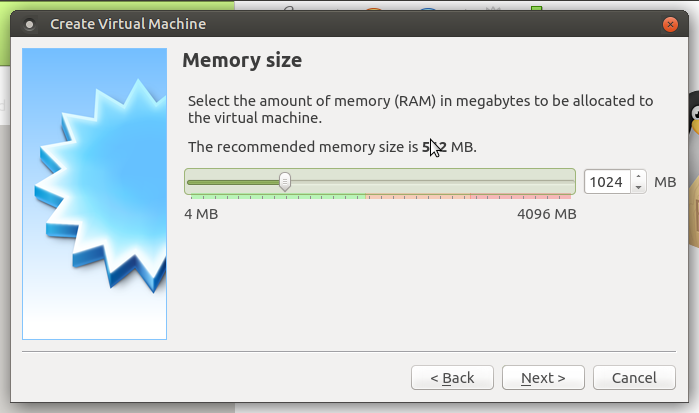
\includegraphics[width=0.752\textwidth]{images/00-02.png}\\[0cm]  
    \caption[Virtual Box]{Virtual Box Memory Size Settings}
    %from \url{http://localhost:3000/}).} % The text in the square bracket is the caption for the list of figures while the text in the curly brackets is the figure caption
    \label{fig:00-03 - Linux Virtual Box Memory Size} 
\end{figure}
Selecting a memory size is the next step. Darkly will not be actively running
as another Virtual Machine would. Therefore only a limited amount of RAM is
required. The recommended size is 512MB but in my opinion I believe 1024MB is
the best.

To set the memory size, a slide is used, as shown in Figure \Vref{fig:00-03 - Linux Virtual Box Memory Size}.

You can also set it using manually by typing in the value.

%---------------------
\subsubsection{Hard Disk File Type}
\begin{figure}[!htb]
    \centering
    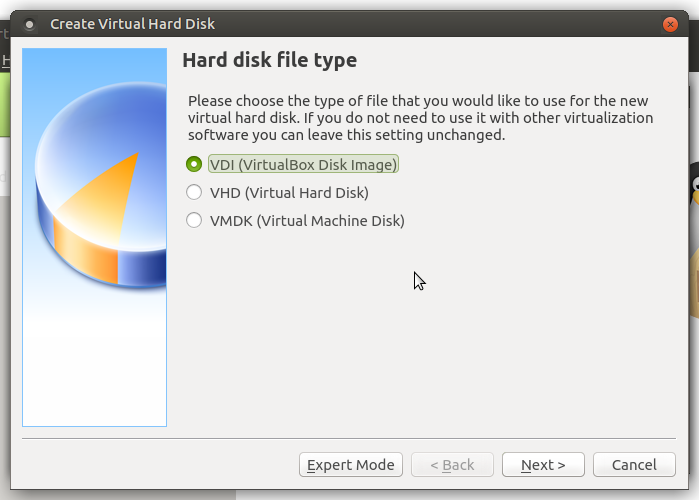
\includegraphics[width=0.752\textwidth]{images/00-03.png}\\[0cm]  
    \caption[Virtual Box]{Virtual Box Disk Type}
    \label{fig:00-04 - Linux Virtual Box Disk Type} 
\end{figure}
Select VirtualBox Disk Image as shown in Figure \Vref{fig:00-04 - Linux Virtual Box Disk Type}.
This is the best decision because the Machine will not be migrated to other
Virtual Machine Players like VMWare etc. The use is short-term.

%---------------------
\subsubsection{Storage Type}
\begin{figure}[!htb]
    \centering
    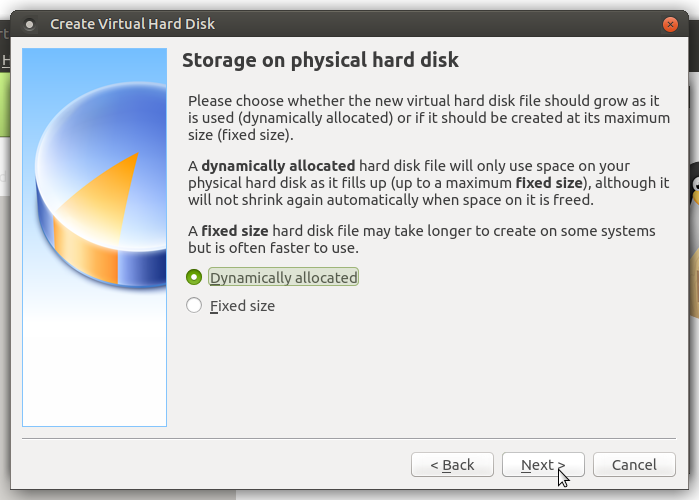
\includegraphics[width=0.752\textwidth]{images/00-04.png}\\[0cm]  
    \caption[Virtual Box]{Virtual Box Storage Type}
    \label{fig:00-05 - Linux Virtual Box Storage Type} 
\end{figure}
Ensure that you have the size Dynamically allocated as shown in Figure \Vref{fig:00-05 - Linux Virtual Box Storage Type}.
If you would like a fixed size, it is okay, but this entails your Hard Disk
being allocated upfront.

Please note, you have not selected your Hard Disk size so it is key to ensure
you are aware of how much space you have free before allocating a fixed space size.

%---------------------
\subsubsection{File Location \& Size}
\begin{figure}[!htb]
    \centering
    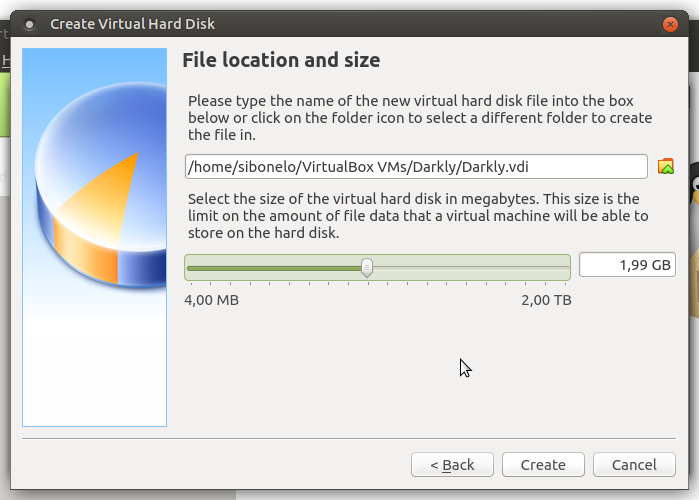
\includegraphics[width=0.752\textwidth]{images/00-05.png}\\[0cm]  
    \caption[Virtual Box]{Virtual Box Hard Disk Location and Size}
    \label{fig:00-06 - Linux Virtual Box Hard Disk} 
\end{figure}
This is where you can set up the location for your Virtual Box Machine to
store its data. Remember that the machine can be stored in one location but
the simulation of its Hard Disk can be stored on a Flash Drive or External
Drive if you wish.\\

I have decided to retain the local drive as the storage location. This is 
the default VirtualBox directory. You can select any size you wish, I have
selected 1,99GB to keep my box small as shown in Figure \Vref{fig:00-06 - Linux Virtual Box Hard Disk}.
I can ammend this later if I need to.

%---------------------
\subsubsection{Mount Disk Image}
%---------------------
\begin{figure}[!htb]
    \centering
    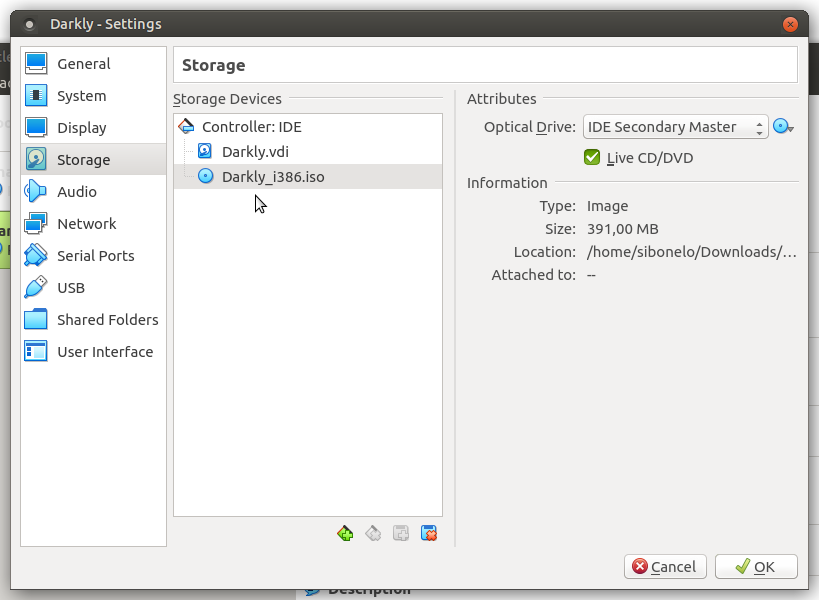
\includegraphics[width=0.752\textwidth]{images/00-06.png}\\[0cm]  
    \caption[Virtual Box]{Virtual Box Settings Navigation}
    \label{fig:00-06 - Linux Virtual Box ISO Mount} 
\end{figure}
\begin{figure}[!htb]
    \centering
    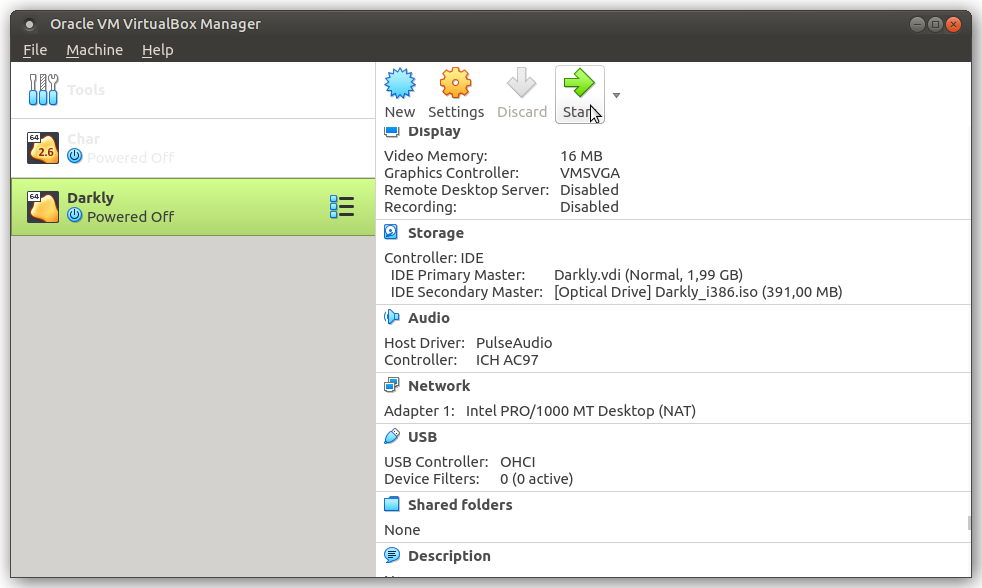
\includegraphics[width=0.752\textwidth]{images/00-07.png}\\[0cm]  
    \caption[Virtual Box]{Virtual Box Setup of Disk Drive Mount Darkly.iso Image}
    \label{fig:00-07 - Linux Virtual Box ISO Mount} 
\end{figure}
The next step is to mount the Darkly.iso disk as a form of storage. Click on
your image 'Darkly' or whatever you may have named it, on the lefthand navigation
panel as shown in Figure \Vref{fig:00-06 - Linux Virtual Box ISO Mount}.\\

Next click on Settings -> Storage -> IDE Secondary Master. After this, navigate
to the folder where the ISO is located. Mount it and you will see it listed
as shown in Figure \Vref{fig:00-07 - Linux Virtual Box ISO Mount}.\\

Click Start (Green arrow pointing right) to commence running the image.

%---------------------
\subsubsection{Run Disk Image}
\begin{figure}[!htb]
    \centering
    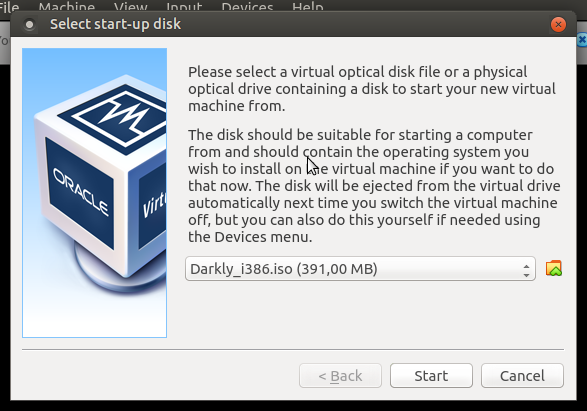
\includegraphics[width=0.752\textwidth]{images/00-08.png}\\[0cm]  
    \caption[Virtual Box]{Virtual Box Start-up Disk Selector}
    \label{fig:00-08 - Linux Virtual Box Startup Disk Selector} 
\end{figure}
As shown in Figure ~\vref{fig:00-08 - Linux Virtual Box Startup Disk Selector},
you are expected to select 'Darkly\_i386.iso' as the start-up disk. This will
then complete the Installation process.

%---------------------
\subsubsection{Running but Incomplete}
\begin{figure}[!htb]
    \centering
    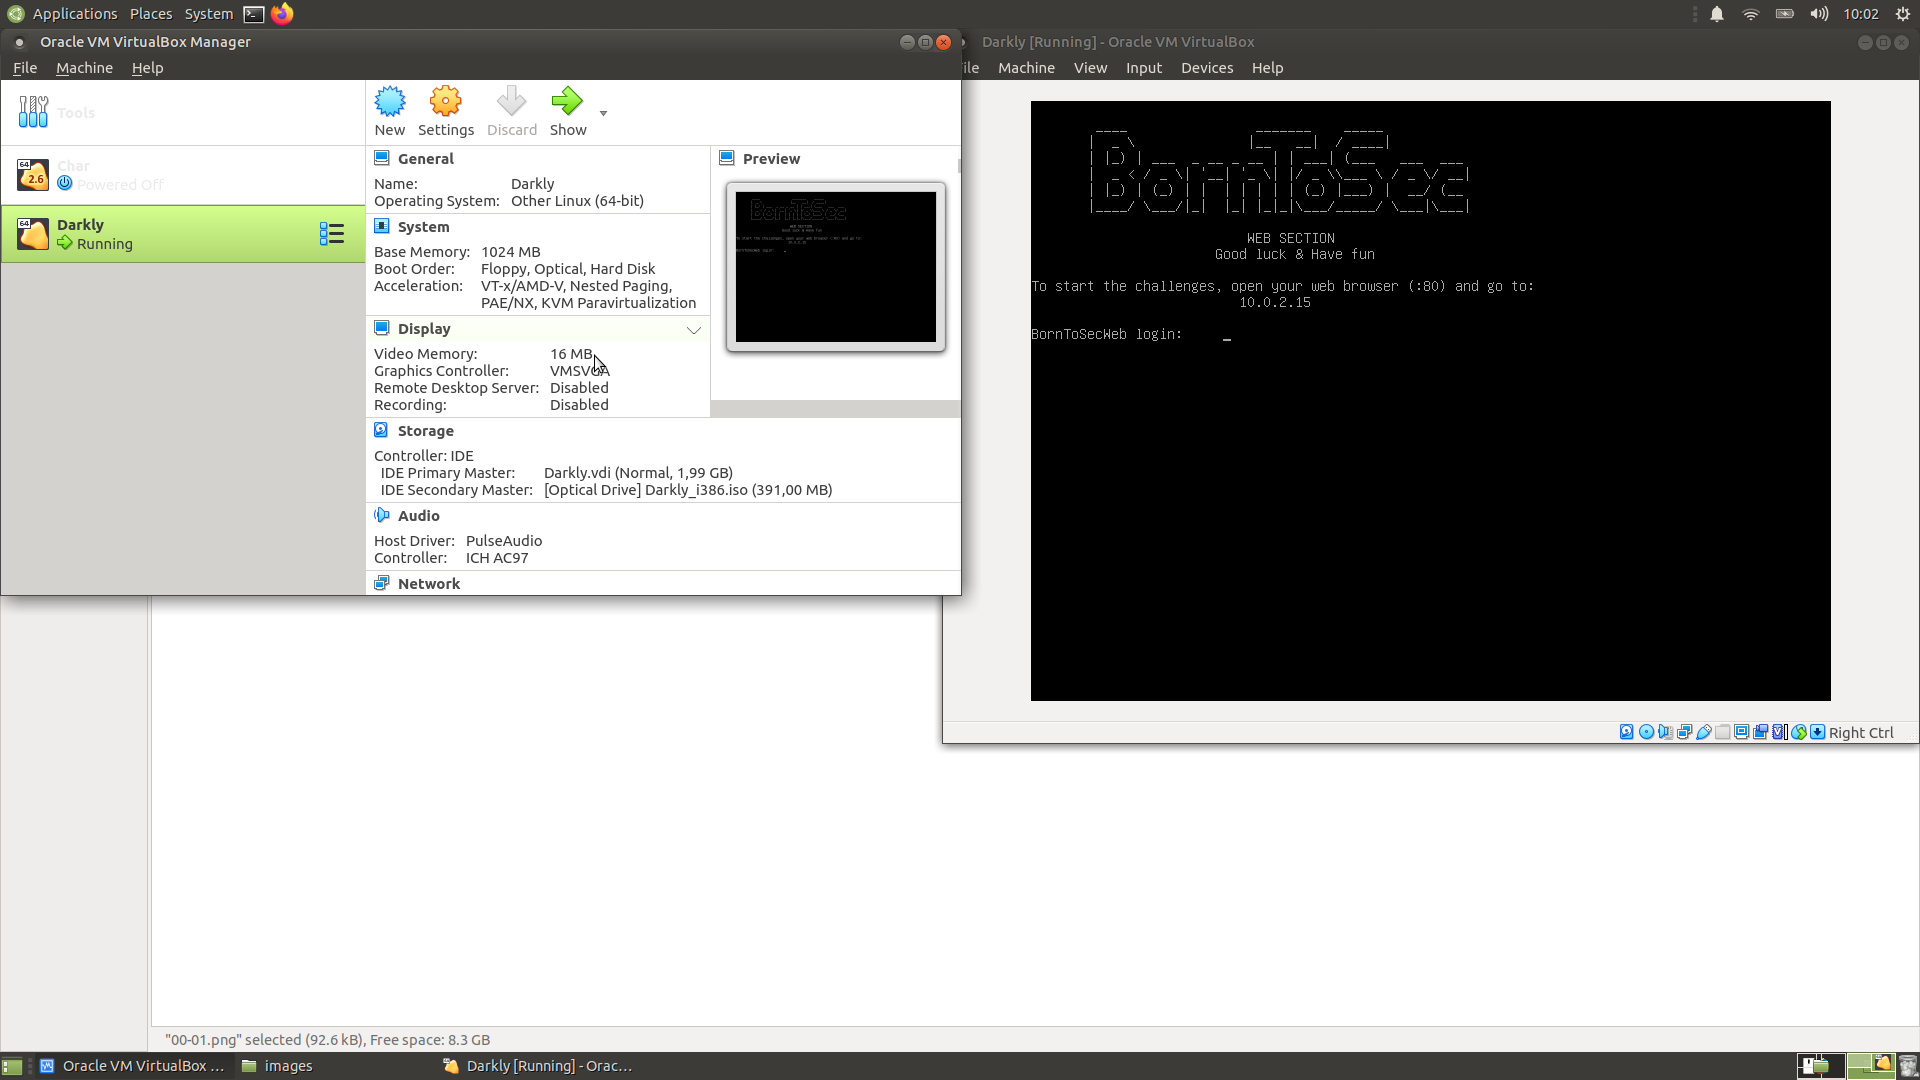
\includegraphics[width=0.752\textwidth]{images/00-09.png}\\[0cm]  
    \caption[Virtual Box]{Darkly ISO running on Ubuntu}
    \label{fig:00-09 - Linux Virtual Box Running not complete} 
\end{figure}
You have successfully installed the VM and it is running. The IP address is
printed on the screen. ...I bet that the IP address does not really work\dots\\

This needs you to go to settings as shown in Figure \vref{fig:00-10 - Linux Virtual Box Set Bridge}

%---------------------
\subsubsection{Set Network Bridge}

\begin{figure}[!htb]
    \centering
    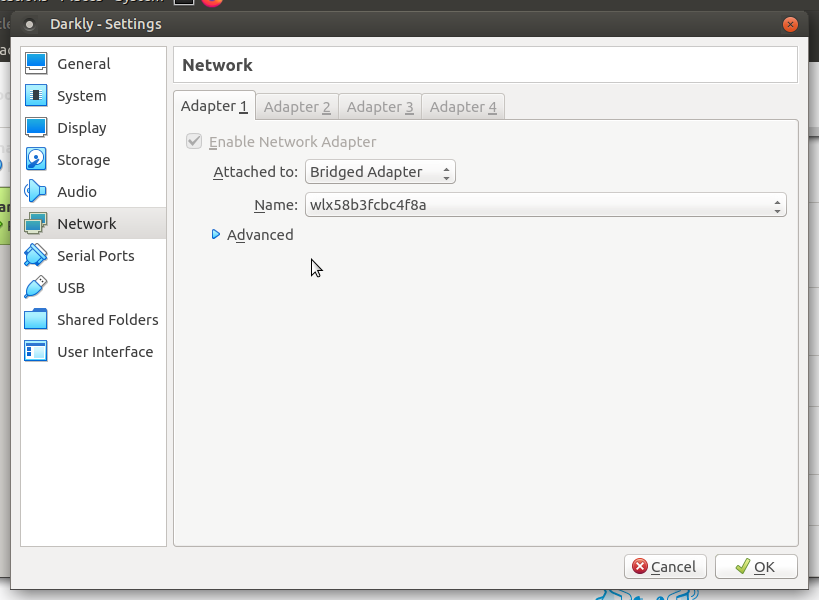
\includegraphics[width=0.752\textwidth]{images/00-10.png}\\[0cm]  
    \caption[Virtual Box]{Set the Network to Bridge not NAT}
    \label{fig:00-10 - Linux Virtual Box Set Bridge} 
\end{figure}
On the lefthand navigation-bar, Select Network -> Adaptor 1.
Change the settings from a NAT Adaptor as would be the default, and set it
to a 'Bridge' connection. as shown in Figure \vref{fig:00-10 - Linux Virtual Box Set Bridge}.

%---------------------
\subsubsection{Don't Panic! Loading Screen}

\begin{figure}[!htb]
    \centering
    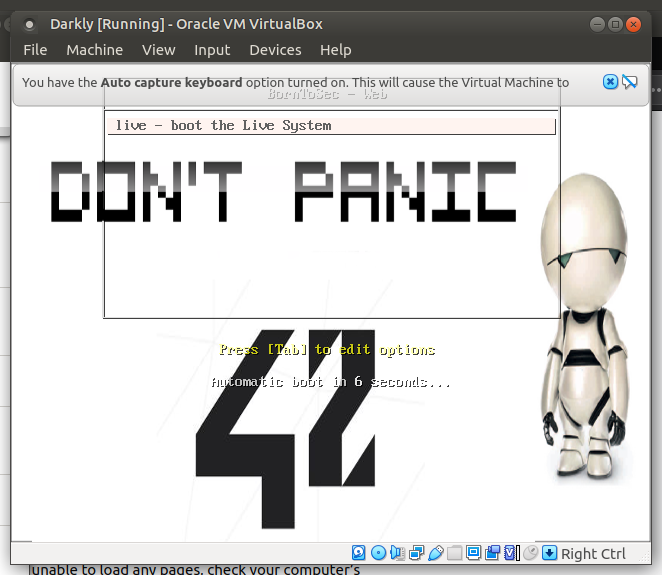
\includegraphics[width=0.752\textwidth]{images/00-11.png}\\[0cm]  
    \caption[Virtual Box]{Virtual Box Loading Screen Splash with Hitchhiker's Guide Robot}
    \label{fig:00-11 - Linux Virtual Box LoadingScreen1} 
\end{figure}
\subparagraph{Don't Panic, it's just a loading screen}

%---------------------
\subsubsection{More Loading Screens}
\begin{figure}[!htb]
    \centering
    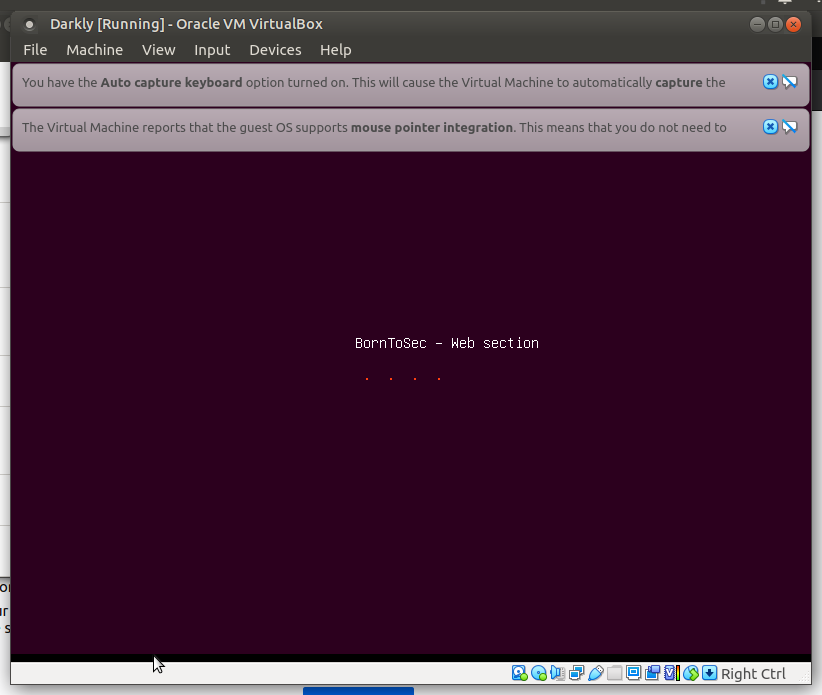
\includegraphics[width=0.752\textwidth]{images/00-12.png}\\[0cm]  
    \caption[Virtual Box]{More Virtual Box Loading Screens}
    \label{fig:00-12 - Linux Virtual Box LoadingScreen2} 
\end{figure}
If you are seeing the figure shown in Figure \vref{fig:00-12 - Linux Virtual Box LoadingScreen2}
you are making good progress and must hang in there.

%---------------------
\subsubsection{Up \& Running}

\begin{figure}[!htb]
    \centering
    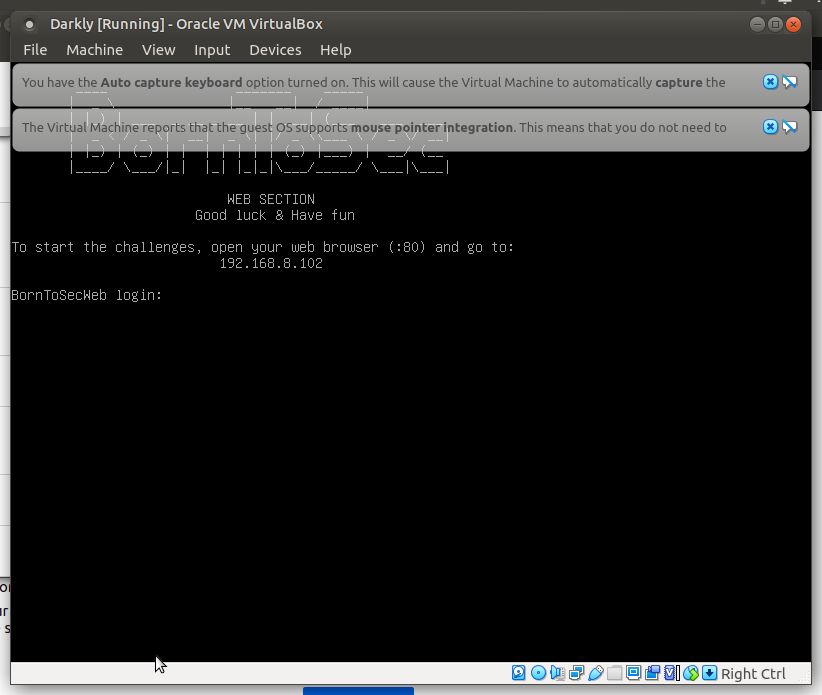
\includegraphics[width=0.752\textwidth]{images/00-13.png}\\[0cm]  
    \caption[Virtual Box]{Virtual Box Fully Loaded Screen with IP Address \& Prompt}
    \label{fig:00-13 - Linux Virtual Box LoadedIP} 

\end{figure}
The new IP Address should look different to the first one and should be similar to
your own IP address after runnung 'ifconfig'.
You should see a similar figure to that shown in Figure \vref{fig:00-13 - Linux Virtual Box LoadedIP}.

%---------------------
\subsubsection{BornToSec}
\begin{figure}[!htb]
    \centering
    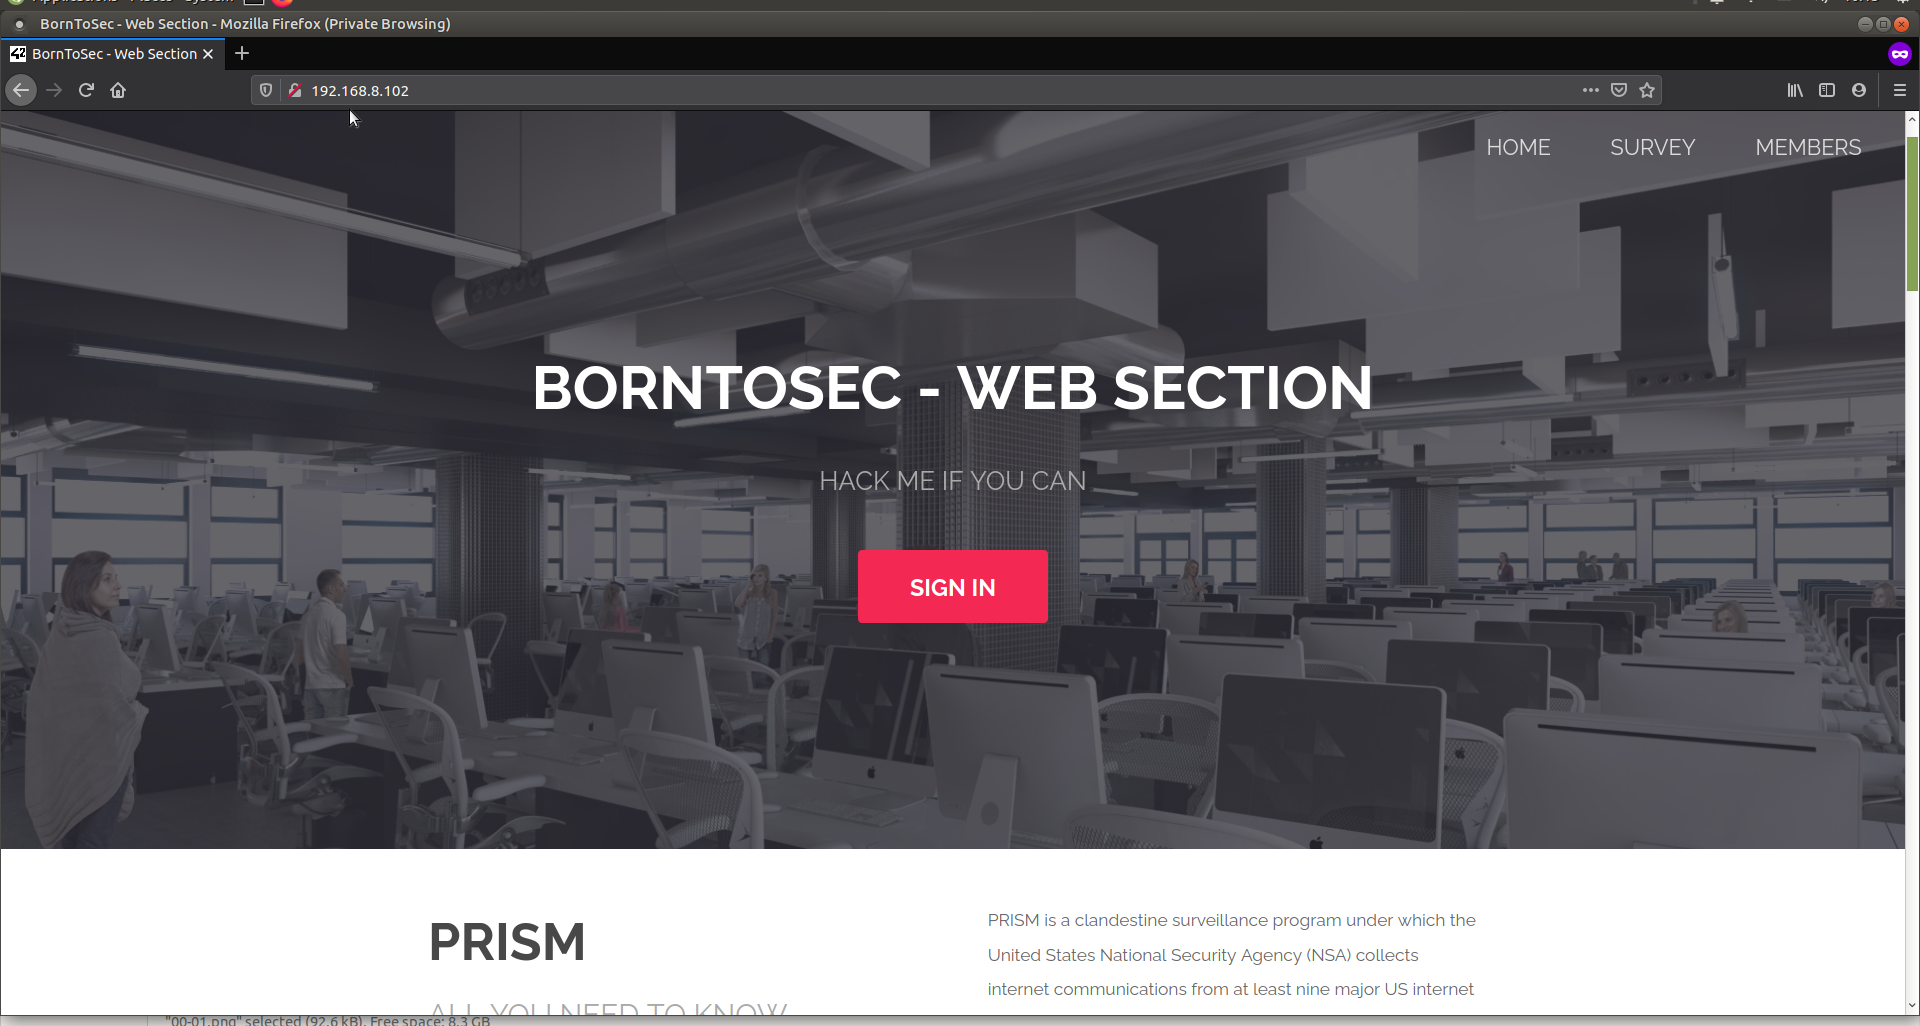
\includegraphics[width=0.752\textwidth]{images/00-14.png}\\[0cm]  
    \caption[Virtual Box]{BornToSec Homepage}
    \label{fig:00-14 - Linux Virtual Box HomePage} 
\end{figure}
If you see the same figure on your screen as the one shown on Figure \vref{fig:00-14 - Linux Virtual Box HomePage},
then you have successfully setup your Virtual Machine.

\paragraph{Time To DO The FUN Stuff!}
